% !TEX root =  paper.tex

\section{Proposed Approach}\label{sec:approach}

\begin{figure}[t]
    \centering
    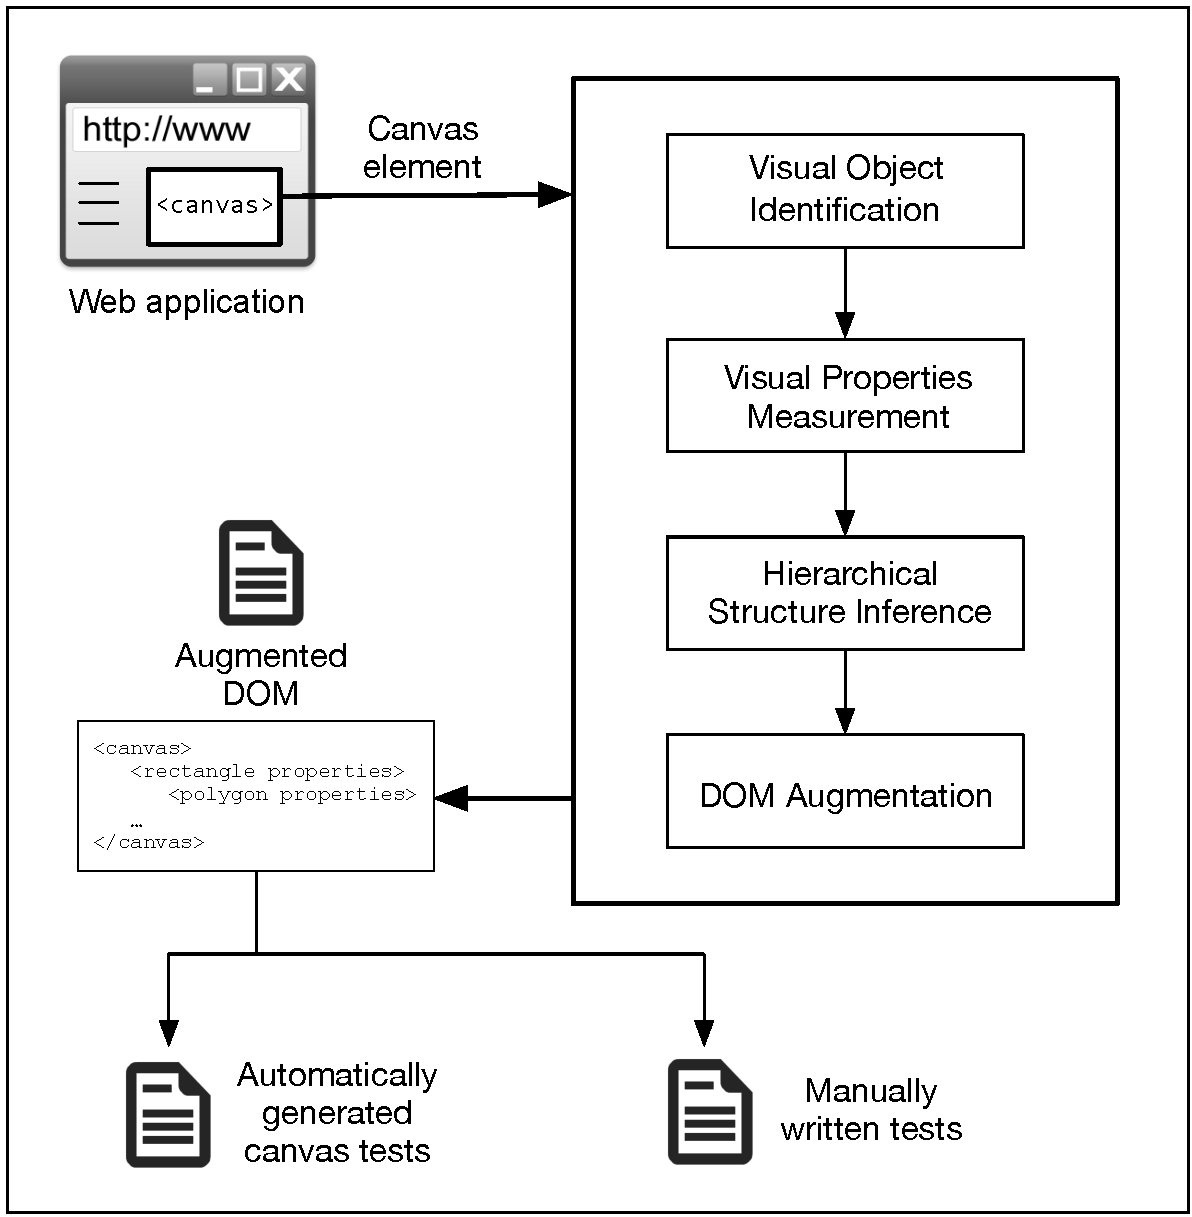
\includegraphics[trim={0.0cm 0.0cm 0.0cm 0.0cm},clip,height=7.9cm,width=0.62\textwidth]{testability/figures/canvasure-overview-figure.pdf}
    \caption{Overview of the proposed approach.}
    \label{fig:approach-overview-1}
\end{figure}

The approach starts by automatically opening the webpage containing canvas elements in an instrumented browser.
It focuses on canvas elements only and is therefore agnostic of the rest of the web application's page.
Therefore, it can analyze canvas elements contained in a larger webpage or canvas applications that are solely composed of a single canvas element.

\subsection{Overview}
Figure \ref{fig:approach-overview-1} depicts an overview of the main steps of the proposed approach.
For each canvas element on the page, a screenshot is captured and visually analyzed.
The visual analysis begins by performing a visual identification of objects on the canvas.
Our object identification is capable of identifying common geometrical shapes supported by the canvas API, such as lines, circles, and rectangles, as well as generic arbitrary shapes.
Next, the approach infers the visual properties such as color, size, and location, for each of the detected visual objects.
A list of all supported properties is shown in Table \ref{tbl:info-provided-by-approach}.
Subsequently, the approach builds a hierarchy information of the visual objects contained in the canvas.
This hierarchy information includes parent-child relations between objects, indicating which objects (if any) are contained inside other objects.
The hierarchy also includes z-order information, which indicates front-to-back arrangement of overlapping objects.

All the information extracted through the previous steps is then represented as an augmented DOM inside the canvas element.
The testing of the canvas is performed by generating assertions from the augmented canvas DOM.
We now describe each of these steps in detail in the following subsections.
 

\subsection{Visual Object Identification}
\label{subsec:viz-identification}
The objective of this stage is to detect and identify objects that are present on a canvas element.
We define an object to be present on the canvas if it is rendered and visible in the current screenshot of the canvas.
However, the approach does not require an object to be fully visible; occlusions and overlaps of multiple objects are allowed.
We apply a number of transformations on a copy of the original canvas image, $\mathbf{C_T}$, in this stage.

\head{Color contrast adjustment}
The goal of this first step is to perform a form of color contrast adjustment of the canvas screenshot.
This is performed in order to enable our analysis to \emph{see} objects more clearly. 

The analysis performs the color contrast adjustment through a \emph{color space conversion} of the canvas screenshot,  $\mathbf{C_T}$.
A color space conversion changes the representation of the colors of the pixels from one representation system to an alternative representation. 

We first need to select a suitable conversion method since several methods exist.
To that end, we perform an empirical examination of the eight most common conversion methods \cite{tooms2016colour}, namely HSV, L*a*b*, L*u*v*, CIE-RGB, XYZ, YUV, YIG, YPbPr, and YCbCr.
Each of these is simply a mathematical formula \cite{tooms2016colour} that changes pixels from one color representation to another. 

We empirically evaluate these conversions on a random set of 20 canvas elements.\footnote{http://corehtml5canvas.com} The results of this empirical examination are shown in Figure \ref{fig:param-est-colorspace}.
The figure shows how much contrast there is in the canvas image when using the different color conversions. The contrast is measured using 
the variance in pixel values. Higher values in the figure indicate  more contrast. Based on the results shown in the figure, the YCbCr conversion yields the best color contrast.
YCbCr will therefore be our choice for the color space that the canvas will be converted to.
Therefore, the algorithm creates a new image, $\mathbf{\bar{C}_T}$, which represents the canvas screenshot in YCbCr.
An example of the outcome of this step is shown in Figure \ref{fig:stages-examples}-a for a part of the motivating example.


\head{Detecting object boundaries}
The goal of this step is to detect the boundary of each object in the canvas.
This is performed in order to allow the analysis to roughly estimate where the objects are in the canvas image; this boundary information is used later to identify objects and their properties.

In order to detect these boundaries, we calculate the image gradient \cite{fernandez2012advanced}.
The image gradient is a mathematical processing applied on the canvas image to extract edges, which are the parts of the canvas where there is a transition from one object to another; for example, a boundary between an object and its background.

First, we need to select a suitable method to calculate the image gradient since several methods exist.
In order to be able to compute more accurate gradients for various canvas object shapes, we use the Scharr method \cite{scharr2000optimal}.
We make this choice because this method has been shown \cite{kroon2009numerical} to yield good results for smooth and curved objects in addition to angled objects.
 This would therefore be suitable for processing objects found on canvas elements.
  We compute the image gradient on $\mathbf{\bar{C}_T}$, and call it $\nabla \mathbf{\bar{C}_T}$.

Next, the analysis performs a binary transformation and converts each pixel in $\nabla \mathbf{\bar{C}_T}$ into either 0 or 1.
 A value of 1 represents a pixel that is on the object boundary, and a value of 0 means otherwise.
  The processed canvas image is called $(\nabla \mathbf{\bar{C}_T})^B$. 
To compute $(\nabla \mathbf{\bar{C}_T})^B$, we need to perform thresholding on the image, i.e., the reduction of a graylevel image to a binary image. 
We choose a machine learning clustering approach called Otsu thresholding from the computer vision literature, to perform this thresholding.
 Otsu's method is clustering-based and has been shown \cite{sezgin2004survey} to yield high performance. The outcome of this step is depicted in Figure \ref{fig:stages-examples}-b for the motivating example. 


\head{Separating objects}
So far, we have a collection of boundaries, but we do not know which group of boundaries belong together as part of the same object.
The goal of this step is to separate the different boundaries detected in the last step. 

\begin{figure}[t]
    \centering
    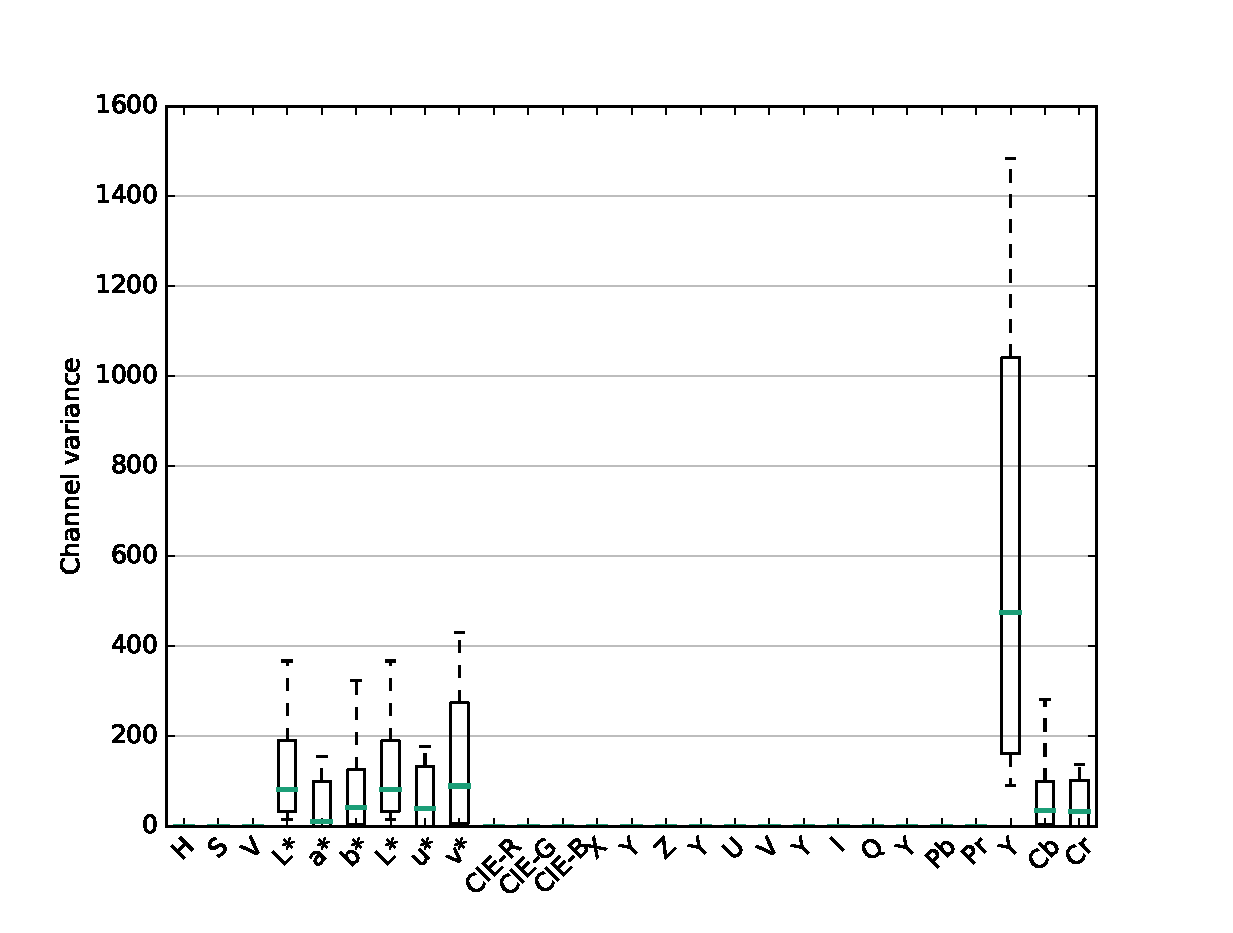
\includegraphics[trim={0.3cm 0.3cm 0.3cm 0.3cm},clip,height=0.35\textheight, width=0.74\textwidth]{testability/figures/colorspace-parameter.eps}
    \caption{Parameter estimation for the color contrast adjustment step of the algorithm. Choosing the YCbCr color representation yields best contrast adjustment for the canvas screenshot. Higher values are better. }
    \label{fig:param-est-colorspace}
\end{figure}



First, our analysis goes through the list of all detected boundaries. For each boundary, the algorithm walks on the boundary, step by step, and examines which other boundaries are connected to it. At the end of this process, we have a group of disjoint boundaries $\mathbf{B}_i$:
%\begin{align}
\begin{equation}
\label{eqn:approach-regions}
(\nabla \mathbf{\bar{C}_T})^B = \bigcup \mathbf{B}_i \,\, : \,\, \bigcap \mathbf{B}_i \equiv \O
\end{equation}
%\end{align}	
where $\mathbf{B}_i$ is a set containing the boundary pixels of the $i^{th}$ detected object in the canvas. The equation shows that each boundary $\mathbf{B}_i$ is separate from other boundaries, $\mathbf{B}_{j\neq i}$.

The algorithm then proceeds by computing the \emph{Euler number} \cite{sossa1996computation} for each boundary $\mathbf{B}_i$. The Euler number is a metric that shows whether a boundary has branches, or is a continuous boundary. For example, geometric shapes such as rectangles or circles have boundaries that continuously surround the shape without branching. On the other hand, two rectangles sharing an edge will have a branch in their boundary.

Next, the algorithm uses the Euler number $\mathcal{E}$ that was just computed in order to check for branching in a boundary. A value of $\mathcal{E} = 0$ indicates that the boundary is one continuous shape without branching. For this case, the algorithm saves the boundary as is without further modifications. On the other hand, a value of $\mathcal{E} < 0$ indicates that a boundary has branching. In this case, the algorithm breaks down the original boundary and creates new boundaries for each branching. We note that this will not cause 
any unnecessary or excessive fragmentation of the structure, 
because the fragmentation only occurs when the boundary branches, 
and no branching occurs for continuous (i.e., unbranched) segments 
of the object.  

At this stage, the analysis has extracted a set of boundaries $\mathbf{B}_i$ from the canvas image that are separate from each other and non-intersecting.  
An example of the outcome of this step is shown in Figure \ref{fig:stages-examples}-c.

\head{Extracting segments on boundaries}
The purpose of this step is to help identify the type of each object (e.g., rectangle, circle, arbitrary shapes, etc) based on extracted segments from its boundary. To this end, we take the object boundaries detected so far and break them into smaller line segments.  Objects that are curved and smooth, such as circles or generic shapes, are still represented by linear segments too, but as minuscule lines at a zoomed-in scale. While more complicated computer graphics models might be used (e.g., curves, polynomials), we opted 
for linear segments to simplify the analysis and make it faster. 

Following the detection of all boundaries $\mathbf{B}_i$, 
we need to understand what the \emph{identity} of each boundary is. 
This is because, at this stage, we only have a collection of boundaries but do not know what shapes do they represent, or 
what their properties are (e.g., dimensions, colors). 
The first step towards gaining this information is to segment these boundaries or break them down into smaller sections. 
Accordingly, the analysis proceeds by populating each boundary with a random set of probabilistic Hough segments from the computer vision literature \cite{matas2000robust}. These segments are small linear portions of the boundary of each region. This approach has been shown \cite{kiryati2000randomized} to produce robust extraction of boundary segments. In essence, this step performs rough clustering of boundary coordinates and groups neighboring points into a set of small segments.

The generated probabilistic segments are, however, often redundant duplicates, overlapping, and/or intersecting. 
This is because the aforementioned Hough segmentation process is stochastic in nature and while it is robust in most situations, its stochastic nature does cause to generate false positives. 
This presents a challenge in terms of identifying which segment is a true linear segment and which is redundant. 
As such, the set of all generated segments does not have a direct 1-to-1 correspondence to linear segments on the boundary.

We address this by performing a post-processing of the generated segments. Post-processing starts by creating an \emph{R-tree} index. An R-tree~\cite{hadjieleftheriou2008r} is a database structure that allows storing, querying, and retrieving data that is spatial in nature (e.g., locations, point sets). Our set of segments is also an example of such spatial data. Therefore, we insert the segments into an R-tree index in order to efficiently perform spatial queries such as finding intersecting segments or neighbors.
 
Accordingly, two sets of operations are performed on the R-tree index. The first operation consists of iterating through each line segment in the index and then querying the existence of other segments with full or partial spatial intersection. The second operation also iterates through each line segment in the index, but queries the existence of neighbouring segments instead of intersections.

For the first R-tree operation, the result of each iteration is a set of segments that are fully or partially intersecting. The algorithm then performs a pair-wise iteration over the intersecting subset. For a pair of line segments that are parallel, the algorithm removes the smaller segment if it is fully enclosed in the larger segment. Otherwise, in cases where the rectangles (which represent the bounding boxes of objects) are partially overlapping, the two parallel segments are merged into one new line segment, and then removed from the set.

\begin{figure}%[b]
    \centering
    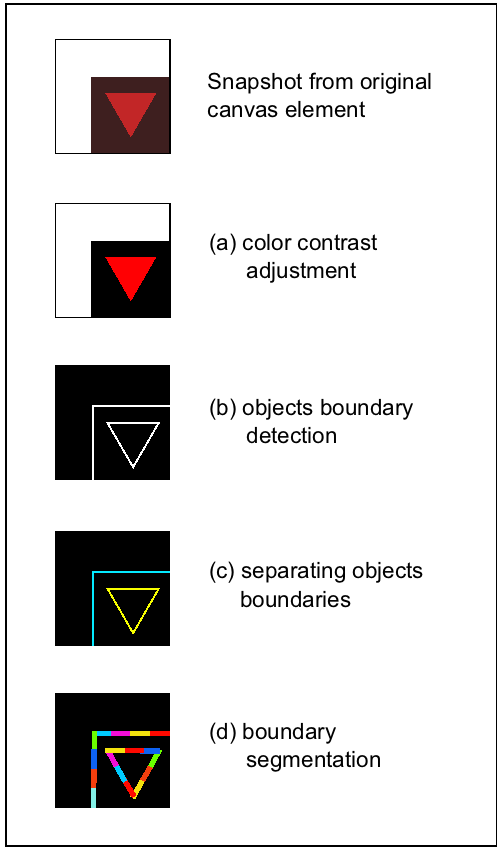
\includegraphics[trim={0.0cm 0.0cm 0.0cm 0.0cm},clip,height=7.5cm,width=0.35\textwidth]{testability/figures/stages-illustration.png}
    \caption{Illustration of the general stages involved in the visual identification of canvas objects. Best viewed on a color monitor. }
    \label{fig:stages-examples}
\end{figure}

For the second R-tree operation, the result of each iteration is a subset of segments that are neighbours of each other. The algorithm forms this subset by querying the R-tree index for the 4 spatial neighbours, one neighbour in each direction, around the query rectangle. The algorithm then performs a pair-wise iteration over the subset. Pairs that are both collinear and parallel are then merged into one new segment, and the forming segments are dropped from the set. Other pairs are left in the set as is.

%\begin{table*}[tb]
\begin{sidewaystable}
\setlength{\tabcolsep}{6pt}
\renewcommand{\arraystretch}{0.9}
\centering
\caption{List of the information that is visually inferred from the screenshots of web canvas elements}
%\begin{tabular}{lccc}
\begin{tabular*}{0.99\textwidth}{l @{\extracolsep{\fill}} ll}
\toprule
\textbf{Visual object identity} &  \textbf{Visual properties}  &  \textbf{Hierarchical structure} \\

\midrule
lines, triangles, rectangles,  &  - centroid: geometric center point of objects & - z-order: relative order of objects \\

squares, circles, & - size: & in the z-direction (i.e. behind or \\

generic shapes (polygons) & \, \, \, - width and height: for rectangles and squares & in front of other objects) \\

 & \, \, \, - diameter: for circles &  \\ 
 
* Note: our approach allows  & - color (HTML hex values) & - Parent-child relation: which \\

multiple overlapping, partially  & - orientation: number of degrees of rotation from horizon & objects are contained inside  \\

visible, or nested combinations & - point-set: the set of points representing generic shapes (polygons) & other objects. \\

of these objects. & & \\ 
 
\bottomrule
%\end{tabular}
\end{tabular*}
\label{tbl:info-provided-by-approach}
%\end{table*} 
\end{sidewaystable}


At this point, we have constructed a final set of line segments for each boundary. The analysis is ready to identify the shape type (e.g., lines, rectangles) of each object. An object whose set of segments has a cardinality of 1 is reported as belonging to the `line' type. Similarly, a set of three connected lines are triangles, and four lines are rectangles. For other objects, the analysis first performs an ellipse fitting to cover the object. Then, the relation between the major and minor axes of the ellipse is computed. If these axes are equal, then the detected shape is identified as a circle if the object's set of line segments has a cardinality of more than 4 (i.e. more than a rectangle) and its area is \emph{solid}. These set of conditions define what a circle is exactly. This is because a  region is defined as \emph{solid} when the the area of that region is identical to the area of the convex hull of the same region. On the other hand, when the region is not solid, the object is identified as a polygon.
Table \ref{tbl:info-provided-by-approach} lists the different object types recognizable by our approach. These types are the same types of objects provided by the canvas API. We note that our approach does not require any training dataset like machine learning approaches, because the attributes and identities of various shapes can be more precisely and robustly captured using mathematical ratios such as the process conducted in this step.
 
\subsection{Visual Properties Measurement}
\label{subsec:viz-props}

At this stage, our technique measures the visual properties of the objects detected in the previous section. These properties are extracted from the original canvas screenshot and include parameters such as location, size, and color. Table \ref{tbl:info-provided-by-approach} shows a list of the visual properties that are measured by the technique for the detected visual objects. This subsection describes the process by which we measure these properties.

\head{Object position} First, the technique calculates the centroid of each detected object. This is done by computing the arithmetic mean of all coordinates in the object. The centroid would therefore represent the point that minimizes the average Euclidean distance between itself and other coordinates in the object.

\head{Color} Next, for all coordinates in the object, the analysis computes the median pixel vector. This is performed to remove outliers that might be present due to small protrusions in the detected region. This vector is then assigned to the color property of the detected object.

\head{Size and orientation}
Subsequently, the analysis performs an ellipse fitting to the region of the object. The ellipse is centred on the centroid, and its axes are fitted so that the ellipse covers the entire object. By the end of this process, an ellipse is generated for each detected object, with each ellipse having a centre, a major axis, and a minor axis. The analysis then extracts a number of visual properties based on the fitted ellipse. First, if the shape is a rectangle, the ellipse axes determine the width and height because the ellipse's major and minor axes would align with the rectangle's axes. If the shape is a circle, then ellipse axes determine the diameter. Next, an orientation is assigned to the object. This orientation is computed as the angle between the major axis of the ellipse and the positive horizontal axis. This represents how much the object is rotated. 


\head{Point set}
Finally, the analysis extracts a representative point set for each object. This point set lists the coordinates necessary to reconstruct the object. This set is only generated for triangles and generic shapes (polygons), since other object categories are fully identified using their other measured properties, as shown in Table \ref{tbl:info-provided-by-approach}. 
In order to generate this representative point set, the analysis takes as input the coordinates of the object boundary and then proceeds to apply the \emph{Harris} operator for the computer vision literature \cite{ryu2011formula}, which is a mathematical transformation that detects points of intersections in boundaries. This process extracts points with more than one directions of lines coming in/out of it, which yields points where linear segments intersect. 
 
\subsection{Hierarchical Structure Inference}

For each detected canvas object, the analysis then performs a sequence of operations on the canvas screenshot that we have processed so far in order to infer any hierarchical information. We define hierarchical information as the information pertaining to the relative spatial relations between overlapping or nested objects. Objects that are not overlapping or nested have no hierarchical information.

More specifically, the hierarchical information of an object has two parts: the z-order and the parent-child relations. 
The z-order determines the relative arrangement of overlapping objects along the z-axis (i.e., front to back arrangement). While the width of the screen is represented with an x axis and the height of the screen represented by a y axis, the z-axis is perpendicular to the xy screen plane and points towards the user. That is, it determines which objects are closer to the viewer and away from the screen, and which are away from the viewer into the screen. 

The second part of hierarchical information is the parent-child relations.
This hierarchical information examines nested objects and determines which are children objects and which objects are their parents.
We define object A to be a child of object B if object A is entirely visually contained inside object B.
Equivalently, object B is a a parent of object A if it entirely contains it.
Objects that are not fully contained in other objects (for example, in cases of partial overlaps) are siblings, and do not have a parent-child relation.

The analysis starts the inference process by creating two directed acyclic graphs for the detected objects.
The first graph, $\mathbf{P}$, captures parent-child information.
The second graph, $\mathbf{Z}$, contains z-order information.
Every object is initialized as a degree zero vertex on the graphs.
Subsequently, the analysis creates an R-tree index. Each item in the index is a 2-tuple of a detected object and its minimum bounding rectangle. 

The analysis then iterates over the collection of detected objects.
For each object, the analysis performs a spatial query on the R-tree to determine the leaves that are intersecting with the object.
This results in one of three possible scenarios.
The first is when the R-tree returns no intersections with the object.
The second is when the intersecting object has its minimal rectangle fully inside the query object.
The third case is when the intersecting rectangles are partially overlapping.

For the first case, the minimal rectangles of the tree leaves are non-intersecting.
This query result indicates that there are no overlapping or nested objects with the current object.
As such, the object has no defined hierarchical information.
The $\mathbf{P}$ and $\mathbf{Z}$ graphs are therefore not updated, and the corresponding vertices of the object remain in their initial state of zero degree.

For the second case, the query indicates that one or more objects are fully contained inside the query object.
Therefore, this constitutes a parent-child relation.
Accordingly, we update both graphs $\mathbf{P}$ and $\mathbf{Z}$.
The update to $\mathbf{P}$ is a new directed edge from the child to the parent.
Similarly, the update to $\mathbf{P}$ is also a directed edge from the child to the parent.

Finally, for the last case, the query returns a partial overlap of the minimal rectangles.
As such, this case would not constitute a parent-child relation.
However, it is still possible for this case to have z-order relations.
Accordingly, the analysis proceeds to detect the presence of a z-order relation.
First, the analysis generates the concave parts of the region.
These parts are the subtraction of the convex hull of the region from the original region.
Next, the analysis performs an element-wise logical XOR between concave parts of the object and the objects with the partially overlapping minimal rectangles.
If the result of the operation is a non-zero region, then a z-order relation exists.
The analysis proceeds by creating a directed edge in $\mathbf{Z}$ from the object with the concave parts to the object that is resulting from the R-tree query.


\subsection{Testing through DOM Augmentation}
\label{subsec:testing-using-dom}
At this stage, the analysis has concluded the process of building information about the identity, properties, and hierarchical structure of the objects on the canvas. The analysis proceeds by casting this information into a DOM tree and augmenting it to the original canvas element.

\head{DOM Augmentation}
First, the analysis creates a DOM node for each detected object on the canvas. The tag name of the node matches the identity of the object. For example, an object that has been identified as a triangle is represented as \verb|<triangle>|, generic shapes (polygons) as \verb|<polygon>| and so on. 

Next, for each node in the DOM, the analysis inserts all the detected attributes pertaining to the identified object (see Table \ref{tbl:info-provided-by-approach} for a full list of attributes). For example, a \verb|diameter| attribute is added to each \verb|<circle>| node.

Finally, the analysis then proceeds by arranging the nodes of the DOM according to the inferred hierarchical information. We recall that the hierarchical information consisted of two parts: the parent-child relations contained in the $\mathbf{P}$ graph, and the z-order relations contained in the $\mathbf{Z}$. For the parent-child relation, the analysis re-orders the nodes of the DOM as to make child nodes in the DOM correspond to child objects on the canvas (as described in the hierarchical structure extraction section). The analysis then adds a \verb|z-order| attribute to each node. A z-order of zero indicates a front-most object, and elements further back have increasing negative values.

\lstdefinelanguage{HTML5}{
	language=html,
	alsoletter={-,=},
	otherkeywords={
		% HTML tags
		<html>, <head>, <title>, </title>, <meta, />, </head>, <body>,
		<canvas, </canvas>, <rectangle, </rectangle>, <triangle, </triangle>, <script>, </script>, </body>, </html>, <!, html>, <style>, </style>, ><
	},  
	ndkeywords={
		% General
		=,
		% HTML attributes
		charset=, id=, center=, color=, z-order=, point-a=, point-b=, point-c=,width=, height=,
		% CSS properties
		border:, transform:, -moz-transform:, transition-duration:, transition-property:, transition-timing-function:, z-order=
	},
	morecomment=[s]{<!--}{-->},
	tag=[s]
}

\begin{lstlisting}[language=HTML5,float=*,caption={The visually inferred augmented DOM for the canvas element of the motivating example (Figure \ref{fig:motivating-example-1} and Listing \ref{lst:motivating-example-1})}, label={lst:augmented-DOM-result}]
	<canvas id="canvasBarChart">
	
	<rectangle center="(191,43)" width="86" height="295" z-order="-1" color="#673C8C">
	<triangle center="(107,43)" point-a="(93,43)" point-b="(114,33)" point-c="(114,55)" z-order="0" color="#41A74D"/>
	</rectangle>
	
	<rectangle center="(166,264)" width="87" height="355" z-order="-1" color="#673B8C">
	<triangle center="(57,264)" point-a="(43,265)" point-b="(64,254)" point-c="(64,276)" z-order="0" color="#41A74D"/>
	</rectangle>
	
	... the rest of the generated DOM ...
	</canvas>
\end{lstlisting}

At this stage, the analysis has finished constructing an augmented DOM tree for the canvas element. An example is shown in Listing \ref{lst:augmented-DOM-result} representing the generated augmented DOM corresponding to the motivating example. As shown in lines 4 and 8 of the listing, a triangle node is located inside a rectangle node in the DOM. This corresponds to the state of the original canvas in Figure \ref{fig:motivating-example-1}, where one can see that a triangle is visually located inside a rectangle.


\head{Testing process}
The proposed canvas DOM augmentation approach was designed to extend and enable the use of DOM testing techniques with canvas elements. As such, it can be used in any testing process that is based on the DOM. For example, through browser automation using Selenium, a test can be written to navigate to a page, click a few buttons, and then finally, through the proposed augmentation approach, assert that the canvas has a vertical red rectangle, for instance. This is similar to the common task performed in DOM tests when the presence of a certain element, say a \verb|<div>| with a certain id, is asserted. 

The inferred augmented DOM is then used to test the canvas element in one of two ways. In the first testing approach, a list of assertions can be automatically generated by default to assert the presence of all nodes of the DOM and their attributes and hierarchy, as shown in Listing \ref{lst:generated-tests}. The generated assertions are broken down into three types of assertions that correspond to the information inferred from the canvas: (a) assertions on the identity of objects, (b) assertions on the properties of objects, and (c) assertions on the hierarchy of objects. The reason for separating assertions into three different layers is twofold. First, this enables pinpointing the cause of assertion failures, as opposed to writing one assertion that asserts the state of the entire canvas as a whole. Second, this strategy gives the user a flexible way of choosing which aspect of the canvas to test. For instance, the user can indicate that they are only interested in testing the presence of objects on the canvas, regardless of position or color. Of course, the user can keep the default option where all attributes are tested. Therefore, instead of just simply reporting that a test has failed, the approach, for example, can report that the test has failed because a triangle was absent or has changed color in the canvas.

Alternatively, in the second testing approach, the augmented DOM can be used in a case where a tester would write specific tests to assert the existence of particular objects, properties, or certain hierarchies of interest. %This would then only test the assertions specified by the tester. 
This use case would, therefore, be more appropriate for scenarios such as test-driven development, for instance.
However, we emphasize that the goal of the proposed approach 
is to provide developers with the \emph{ability} to test canvas elements, since they are not testable at the moment. That goal is the priority, more so than providing a complete end to end testing 
solution that would cover all the possible ways or markups 
that developers would prefer to write their tests in. 

     \begin{lstlisting}[language=Java, float=*, caption={The automatically generated test assertions for the canvas element of the motivating example (Figure \ref{fig:motivating-example-1} and Listing \ref{lst:motivating-example-1})}, label={lst:generated-tests}]
// High-level test: testing the identity of objects in the canvas
 assertTrue("'canvasBarChart' should contain 5 triangles",
   webDriver.findElements(By.xpath("//canvas[@id='canvasBarChart']//triangle")).size() == 5);

 assertTrue("'canvasBarChart' should contain 5 rectangles",
   webDriver.findElements(By.xpath("//canvas[@id='canvasBarChart']//rectangle")).size() == 5);
   // ...

// More detailed test: testing the locations of objects in the canvas
 assertNotNull("'canvasBarChart' should contain a triangle at (107,43)",
   webDriver.findElement(By.xpath("//canvas[@id='canvasBarChart']//triangle[@center='(107,43)']")));
	// ...

// More detailed test: testing the size of objects in the canvas
 assertNotNull("'canvasBarChart' should contain a rectangle with width=86 and height=295",
   webDriver.findElement(By.xpath("//canvas[@id='canvasBarChart']//rectangle[@width='86' and @height='295']")));
	// ...

// ... Tests for other properties (z-order, color, etc)
     \end{lstlisting}
	

\header{Implementation}
We implemented our canvas visual inference approach in a tool called \tool\cite{canvasure}. \tool is implemented in Python 3. We use the numpy~\cite{walt2011numpy} library to import basic mathematical and numerical functions, and use the scipy~\cite{jones2014scipy} library for matrix computations on the screenshots. We use the Selenium web driver to run and instrument web applications and extract canvas elements.


